\chapter{Convolution Fundamentals}
\label{ch:conv}

\chapmeta{Beginner}{$\sim$5\,h (3\,h theory + 2\,h practical)}{EuroSAT; synthetic images}

\begin{objbox}
\begin{itemize}[leftmargin=1.2em,nosep]
  \item Define discrete 2D convolution and distinguish it from cross-correlation.
  \item Implement convolution from scratch in NumPy and reproduce \texttt{nn.Conv2d}.
  \item Derive the output-size formula for arbitrary kernel, stride and padding.
  \item Understand kernels, feature maps, weight sharing and the receptive field.
  \item Read and reason about every argument of \texttt{torch.nn.Conv2d}.
\end{itemize}
\end{objbox}

\section{The convolution operation}

A convolution slides a small array of learnable weights --- the \emph{kernel}
or \emph{filter} $K$ --- across an input image $I$ and, at each position,
computes the sum of element-wise products. The result is a \emph{feature map}.
For a single-channel input of size $H\times W$ and a kernel of size
$k\times k$, the (valid) output at position $(i,j)$ is
\begin{equation}
S[i,j] \;=\; (I * K)[i,j] \;=\; \sum_{m=0}^{k-1}\sum_{n=0}^{k-1} K[m,n]\,I[i+m,\,j+n].
\label{eq:conv}
\end{equation}
Figure~\ref{fig:conv} illustrates one such dot-product for a vertical-edge
kernel.

\begin{figure}[h]
\centering
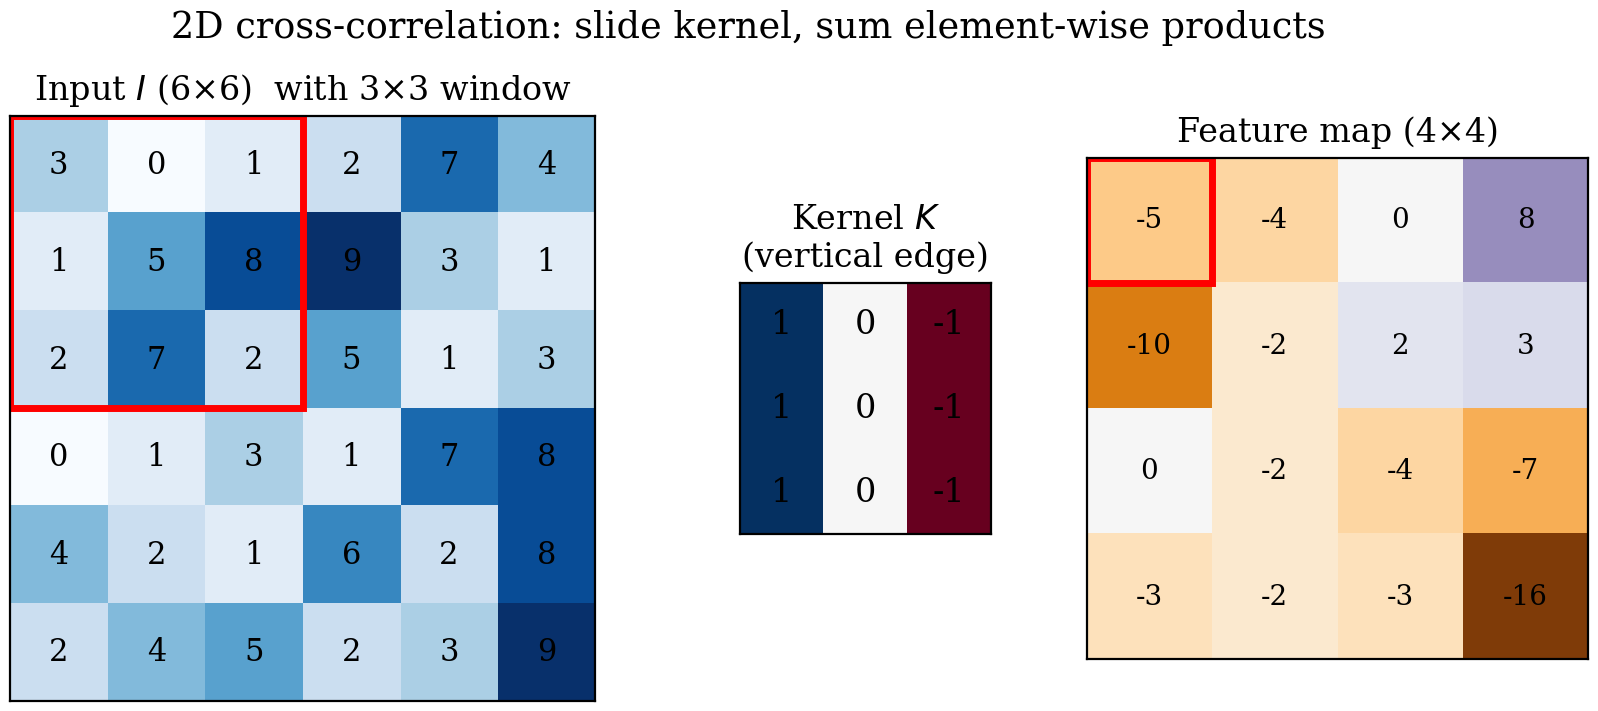
\includegraphics[width=\linewidth]{figures/convolution.png}
\caption{Discrete 2D cross-correlation. The $3\times3$ kernel (centre) is placed
at every valid position of the input (left); each placement produces one output
value (right). The same kernel is reused everywhere --- \emph{weight sharing}.}
\label{fig:conv}
\end{figure}

\paragraph{Convolution vs.\ cross-correlation.}
The mathematical convolution flips the kernel before sliding:
$(I*K)[i,j]=\sum_{m,n}K[m,n]\,I[i-m,j-n]$. Deep-learning frameworks omit the
flip and implement Eq.~\eqref{eq:conv} --- technically \emph{cross-correlation}
--- but call it ``convolution''. Because the kernel weights are learned, the
flip is irrelevant: the network simply learns the un-flipped kernel. We follow
the framework convention throughout.

\paragraph{Multi-channel convolution.}
Real inputs have $C_\mathrm{in}$ channels (3 for RGB, 13 for Sentinel-2). A
single filter then has shape $(C_\mathrm{in},k,k)$ and sums over channels; a
layer learns $C_\mathrm{out}$ such filters, producing $C_\mathrm{out}$ feature
maps:
\begin{equation}
S_o[i,j] \;=\; b_o + \sum_{c=0}^{C_\mathrm{in}-1}\sum_{m=0}^{k-1}\sum_{n=0}^{k-1}
K_o[c,m,n]\,I[c,\,i+m,\,j+n], \qquad o = 0,\dots,C_\mathrm{out}-1.
\label{eq:convmc}
\end{equation}
The weight tensor of a layer therefore has shape
$(C_\mathrm{out},C_\mathrm{in},k,k)$ and the bias has shape $(C_\mathrm{out})$.

\paragraph{Why weight sharing matters.}
A fully connected layer mapping a $64\times64\times3$ image to even $64$
hidden units needs $64\times64\times3\times64 \approx 786{,}000$ weights and is
not translation-equivariant. A convolution with $64$ filters of size
$3\times3\times3$ needs $64\times27 = 1{,}728$ weights, applies the \emph{same}
detector everywhere, and is translation-equivariant by construction. This
parameter economy and built-in spatial prior are why CNNs dominate imagery.

\section{Classic kernels: what filters detect}

Before learned filters, image processing used hand-designed kernels. They build
intuition for what a CNN's early layers discover on their own.
Figure~\ref{fig:kernels} applies several to a synthetic satellite-like scene.

\begin{figure}[h]
\centering
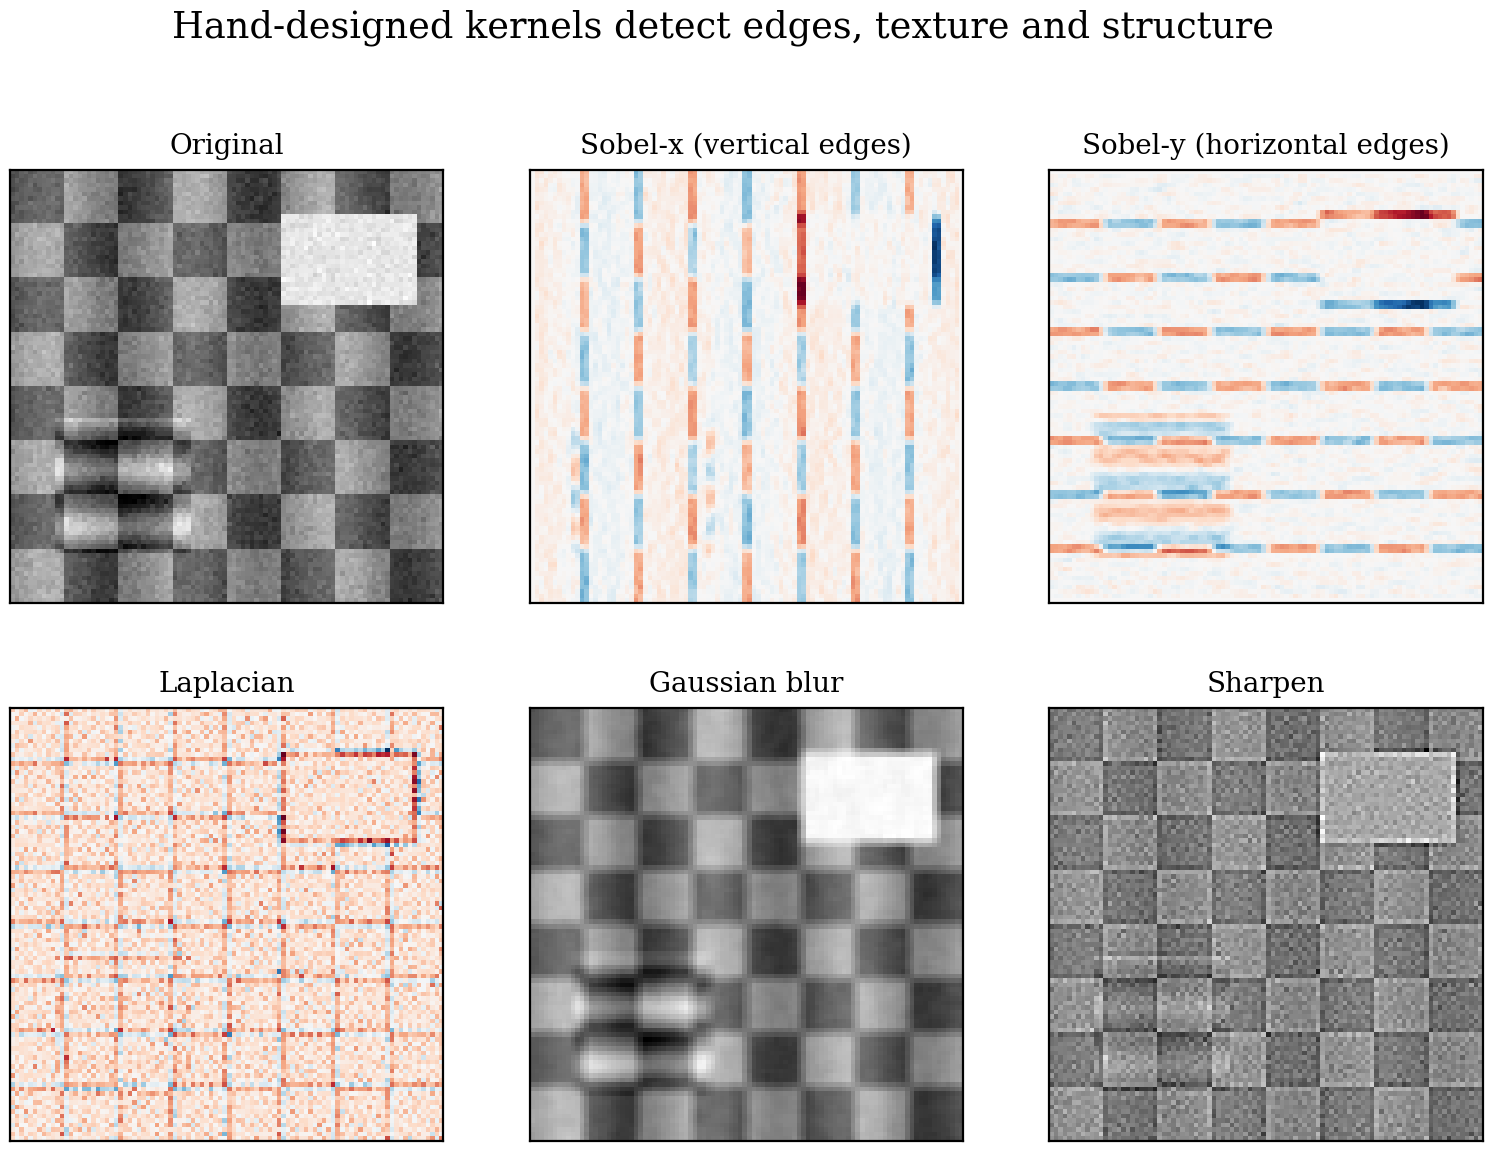
\includegraphics[width=0.95\linewidth]{figures/kernels.png}
\caption{Hand-designed kernels. Sobel filters respond to oriented edges; the
Laplacian to second-order intensity changes; Gaussian blurs; sharpening
amplifies high frequencies. Trained CNN first layers typically rediscover
edge/blob/colour-opponent filters resembling these.}
\label{fig:kernels}
\end{figure}

The horizontal Sobel kernel is
$K=\begin{psmallmatrix}1&0&-1\\2&0&-2\\1&0&-1\end{psmallmatrix}$; it
approximates $\partial I/\partial x$ and fires on vertical edges. Early CNN
layers learn Gabor-like oriented edge and colour-opponent detectors; deeper
layers combine these into textures, object parts and, eventually, semantic
concepts --- a learned hierarchy of the hand-built filters above.

\section{Padding and stride}

\paragraph{Padding.} Valid convolution shrinks the output: each spatial
dimension loses $k-1$ pixels. To keep the spatial size constant (``same''
padding) we pad the border with $p=\lfloor k/2\rfloor$ zeros on each side.

\paragraph{Stride.} The stride $s$ is the step between kernel placements. A
stride of 2 halves the output resolution, providing a learnable alternative to
pooling for downsampling.

\paragraph{Output-size formula.} For input size $n$, kernel $k$, padding $p$,
stride $s$:
\begin{equation}
n_\mathrm{out} = \left\lfloor \frac{n + 2p - k}{s} \right\rfloor + 1.
\label{eq:outsize}
\end{equation}
For $n=64$, $k=3$, $s=1$: $p=0$ gives $62$ (shrinks); $p=1$ gives $64$ (same).
With $s=2$, $k=3$, $p=1$: $n_\mathrm{out}=32$. Memorising
Eq.~\eqref{eq:outsize} prevents the most common shape-mismatch bugs.

\section{The receptive field}

The \emph{receptive field} (RF) of a unit is the region of the input image that
can influence its activation. For $N$ stacked $k\times k$ convolutions with
stride 1 and no pooling,
\begin{equation}
\mathrm{RF}_N = 1 + N\,(k-1).
\label{eq:rf}
\end{equation}
For $3\times3$ kernels: one layer sees $3$, two layers $5$, five layers $9$,
ten layers $19$. Stacking small kernels is cheaper than one large kernel for the
same RF (two $3\times3$ layers, $18$ weights/channel, match one $5\times5$,
$25$ weights) and inserts an extra non-linearity --- the design principle behind
VGG (Chapter~\ref{ch:arch}). Pooling or strided convolution multiplies the RF
growth rate (Figure~\ref{fig:rf}).

\begin{figure}[h]
\centering
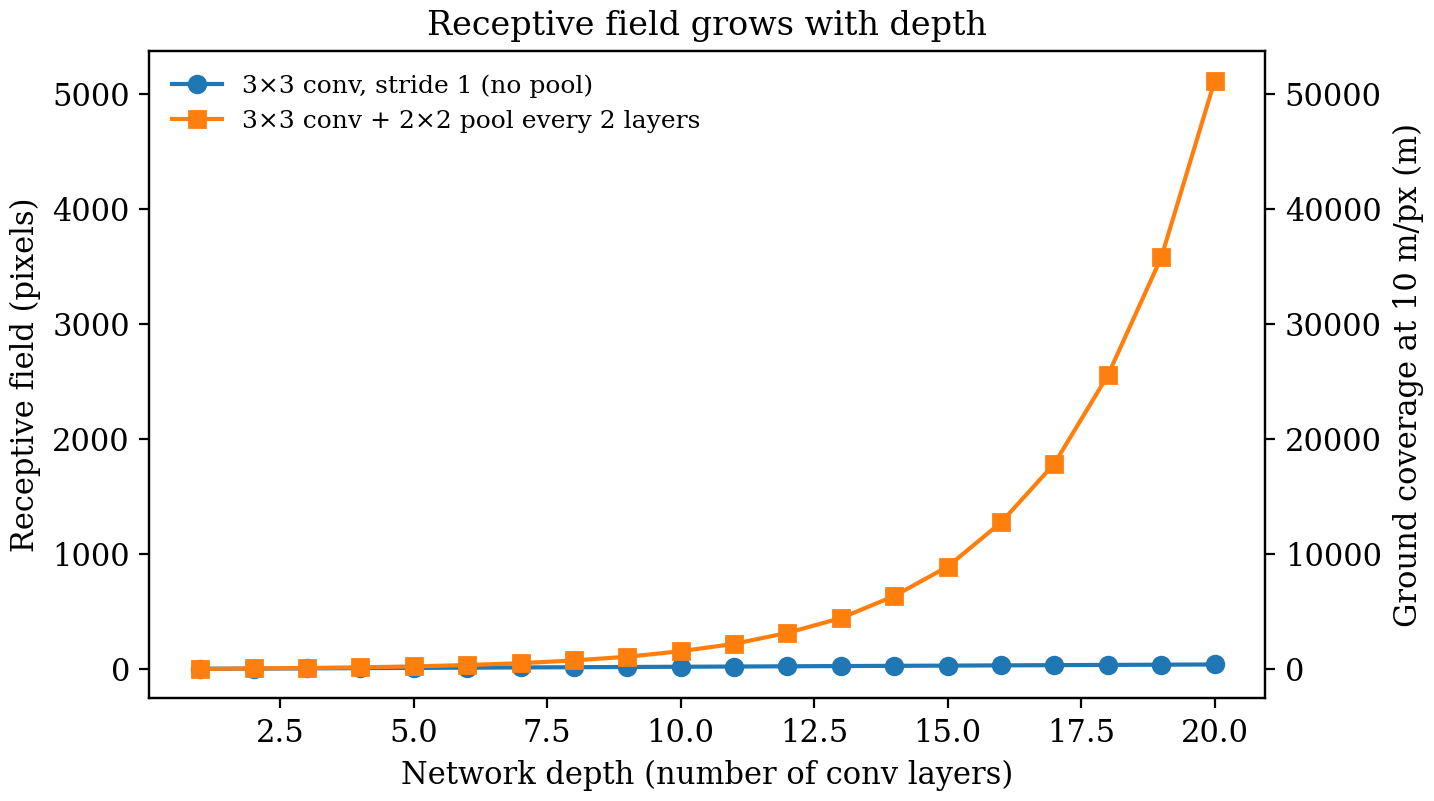
\includegraphics[width=0.72\linewidth]{figures/receptive_field.png}
\caption{Receptive field vs depth. Downsampling layers (pooling or stride~2)
make the RF grow geometrically, letting deep layers ``see'' large ground areas.
At 10\,m/px an RF of $\sim$100\,px corresponds to $\sim$1\,km --- enough to
capture field boundaries and urban blocks.}
\label{fig:rf}
\end{figure}

This is why depth lets a network detect larger objects: a unit in a deep layer
integrates information over a wide spatial extent. For EO this maps directly to
ground distance: matching the RF to the scale of your target features (a road
vs a city) is a real design decision.

\section{\texttt{nn.Conv2d} in PyTorch}

The framework layer realises Eq.~\eqref{eq:convmc}:
\begin{lstlisting}
import torch.nn as nn
conv = nn.Conv2d(in_channels=3, out_channels=32, kernel_size=3,
                 stride=1, padding=1, bias=True)
# weight shape: (out_channels, in_channels, kH, kW) = (32, 3, 3, 3)
# params: out*in*kH*kW + out = 32*3*3*3 + 32 = 896
\end{lstlisting}
Key arguments: \texttt{in\_channels} (input feature maps), \texttt{out\_channels}
(number of filters learned $=$ output maps), \texttt{kernel\_size},
\texttt{stride}, \texttt{padding}, and \texttt{bias} (set \texttt{False} when a
BatchNorm layer follows, since BN has its own shift). The parameter count of a
layer is $C_\mathrm{out}(C_\mathrm{in}\,k^2)+C_\mathrm{out}$; its cost in
multiply--accumulate operations for an $H\times W$ output is
$C_\mathrm{out}C_\mathrm{in}k^2 HW$.

\begin{keybox}
\begin{itemize}[leftmargin=1.2em,nosep]
  \item Convolution = slide kernel, sum element-wise products (Eq.~\ref{eq:conv}); frameworks skip the flip.
  \item A layer learns $C_\mathrm{out}$ filters of shape $(C_\mathrm{in},k,k)$; weight sharing gives translation equivariance and few parameters.
  \item Output size: $\lfloor(n+2p-k)/s\rfloor+1$. Same padding: $p=\lfloor k/2\rfloor$.
  \item Receptive field grows with depth (Eq.~\ref{eq:rf}); pooling/stride accelerate it.
  \item Stacked $3\times3$ convolutions beat one large kernel: fewer params, more non-linearity.
\end{itemize}
\end{keybox}

\begin{practbox}
Notebook: \nbpath{chapter\_02\_convolution\_fundamentals/02\_practical\_convolution\_from\_scratch.ipynb}.
\begin{enumerate}[leftmargin=1.4em,nosep]
  \item Implement \texttt{convolve2d\_numpy(img, kernel)} for valid convolution and
  verify it against \texttt{scipy.signal.correlate2d}.
  \item Apply Sobel-x, Sobel-y, Laplacian, Gaussian-blur and sharpen kernels to an
  EuroSAT sample; display the feature maps.
  \item Verify Eq.~\eqref{eq:outsize} empirically for several $(k,p,s)$ triples.
  \item Recreate the NumPy convolution with \texttt{nn.Conv2d} by manually setting
  its \texttt{weight}; confirm the outputs match.
  \item Trace the receptive field of a 5-layer stack using Eq.~\eqref{eq:rf}.
\end{enumerate}
\begin{lstlisting}
import numpy as np
from numpy.lib.stride_tricks import sliding_window_view
def convolve2d_numpy(img, k):
    win = sliding_window_view(img, k.shape)      # (H-k+1, W-k+1, k, k)
    return np.einsum("ijmn,mn->ij", win, k)
\end{lstlisting}
\end{practbox}

\begin{exbox}
\textbf{2.1 Strided convolution.} Extend \texttt{convolve2d\_numpy} to support
\texttt{stride>1}; verify the output size against Eq.~\eqref{eq:outsize}.\\[2pt]
\textbf{2.2 Parameter \& MAC counting.} For each layer of the
Chapter~\ref{ch:blocks} \texttt{SimpleCNN}, compute learnable parameters and
multiply--accumulates for a $64\times64$ input
($\text{MACs}=C_\mathrm{out}C_\mathrm{in}k^2 H_\mathrm{out}W_\mathrm{out}$).\\[2pt]
\textbf{2.3 Kernel visualisation.} Train \texttt{SimpleCNN} for two epochs
(Chapter~\ref{ch:classif} code) and display the 32 first-layer filters; compare
with random initialisation. Do Gabor-like patterns emerge?\\[2pt]
\textbf{Mini-project.} Hand-design three $3\times3$ kernels detecting (i)
diagonal edges, (ii) a regular grid texture, (iii) a colour-difference response
across channels; apply them to five EuroSAT samples and interpret the maps.
\end{exbox}
